\documentclass[10pt, compress]{beamer}

\usetheme{metropolis}           % Use metropolis theme

\usepackage[export]{adjustbox}
\usepackage{booktabs}
\usepackage[scale=2]{ccicons}
\usefonttheme[onlymath]{serif}

%\usemintedstyle{trac}

\title{Interactive Bayesian Hierarchical Clustering}
\subtitle{}
\date{June 22, 2016}
\author{Sharad Vikram and Sanjoy Dasgupta\\\texttt{\{svikram, dasgupta\}@cs.ucsd.edu}}
\institute{UCSD}

%\setcounter{tocdepth}{1}

\begin{document}

\maketitle

%\section{Background}

%\subsection{Clustering}

\begin{frame}{Hierarchical clustering}
  In \alert{hierarchical clustering}, data
  is recursively partitioned to form a tree (typically binary),
  also called a hierarchy.

  \begin{center}
    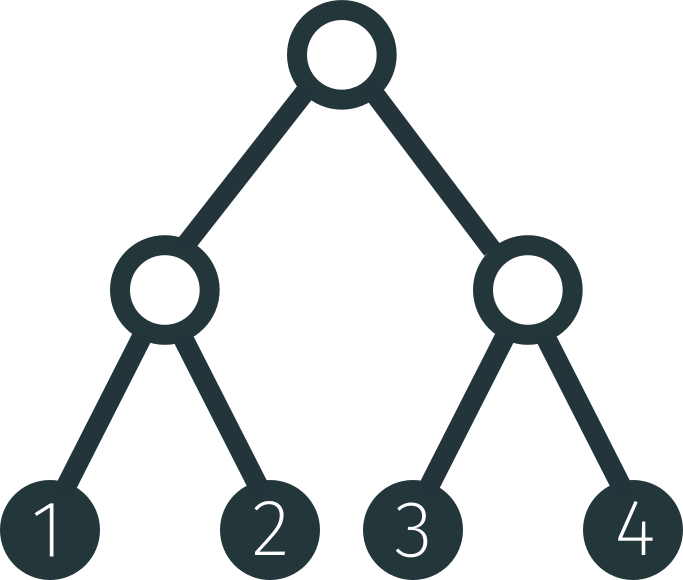
\includegraphics[width=0.5\textwidth]{img/tree-1234-balanced}
  \end{center}

  \pause

Traditional algorithms are \emph{agglomerative}
and \emph{divisive}.

\end{frame}

\begin{frame}{Ambiguous data}
  Consider the two following scenarios where
  circles represent tight clusters of data.

  \begin{center}
    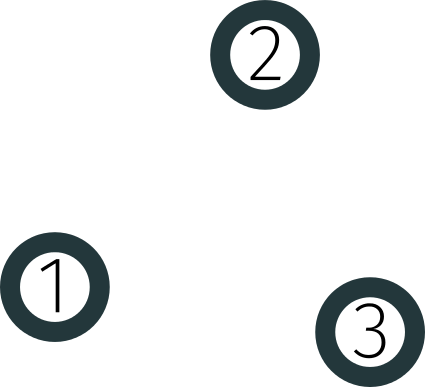
\includegraphics[width=0.3\textwidth]{img/3-cluster}\hfill
    \includegraphics[width=0.45\textwidth]{img/3-cluster-line}
  \end{center}

  \pause
  \textbf{User interaction can help clear up ambiguity!}

\end{frame}

\begin{frame}{Interactive hierarchical clustering}
  \begin{center}
    \includegraphics<1>[width=\textwidth]{img/interaction-0}
    \includegraphics<2>[width=\textwidth]{img/interaction-1}
    \includegraphics<3>[width=\textwidth]{img/interaction-2}
    \includegraphics<4->[width=\textwidth]{img/interaction-3}
  \end{center}
  \begin{itemize}
    \item<4-> User provides a \alert{triplet}. $a$ and $b$
  should be in a subtree together without $c$.
    \item<5-> We show the user the induced tree on the subset of the data $T|_S$.
  \end{itemize}
\end{frame}

\begin{frame}{Bayesian hierarchical clustering}
  We desire a probability distribution over all possible
  trees that explain the data.

  \begin{center}
    \includegraphics<2>[width=0.7\textwidth]{img/3-cluster-distribution.png}
    \includegraphics<3>[width=0.7\textwidth]{img/3-cluster-linear-distribution.png}
  \end{center}
\end{frame}

\begin{frame}{Bayesian hierarchical clustering}
  Define a generative model for the data.
  \begin{itemize}
    \item<1->   Prior distribution $P(T)$, (Dirichlet diffusion tree,
      Kingman's coalescent)
    \item<3->   Likelihood model $P(\theta | T), P(X | T, \theta)$, (Brownian motion,
      Dirichlet-multinomial diffusion)
  %\begin{center}
    %\includegraphics<2>[width=\textwidth]{img/diffusion-1}
    %\includegraphics<3>[width=\textwidth]{img/diffusion-2}
    %\includegraphics<4>[width=\textwidth]{img/diffusion-3}
    %\includegraphics<5>[width=\textwidth]{img/diffusion-4}
  %\end{center}
  \end{itemize}

  \begin{center}
    \includegraphics<2-3>[width=\textwidth]{img/tree-data-0}
    \includegraphics<4>[width=\textwidth]{img/tree-data-1}
  \end{center}

\end{frame}

\begin{frame}{Inference}
  We are interested in the posterior distribution
  $P(T | X)$, which we compute
  via approximate methods like Metropolis-Hastings.

  \uncover<2->{A popular proposal distribution is \alert{subtree-prune
  and regraft} (SPR).}

  \begin{center}
    \includegraphics<3>[width=\textwidth]{img/spr-1}
    \includegraphics<4>[width=\textwidth]{img/spr-2}
    \includegraphics<5->[width=\textwidth]{img/spr-3}
  \end{center}

  \uncover<6->{Parameters $\theta$ can be sampled via Gibbs sampling
  or integrated out via belief propagation.}

\end{frame}

\begin{frame}{Incorporating triplet feedback}

  Recall the interaction model.

  \begin{center}
    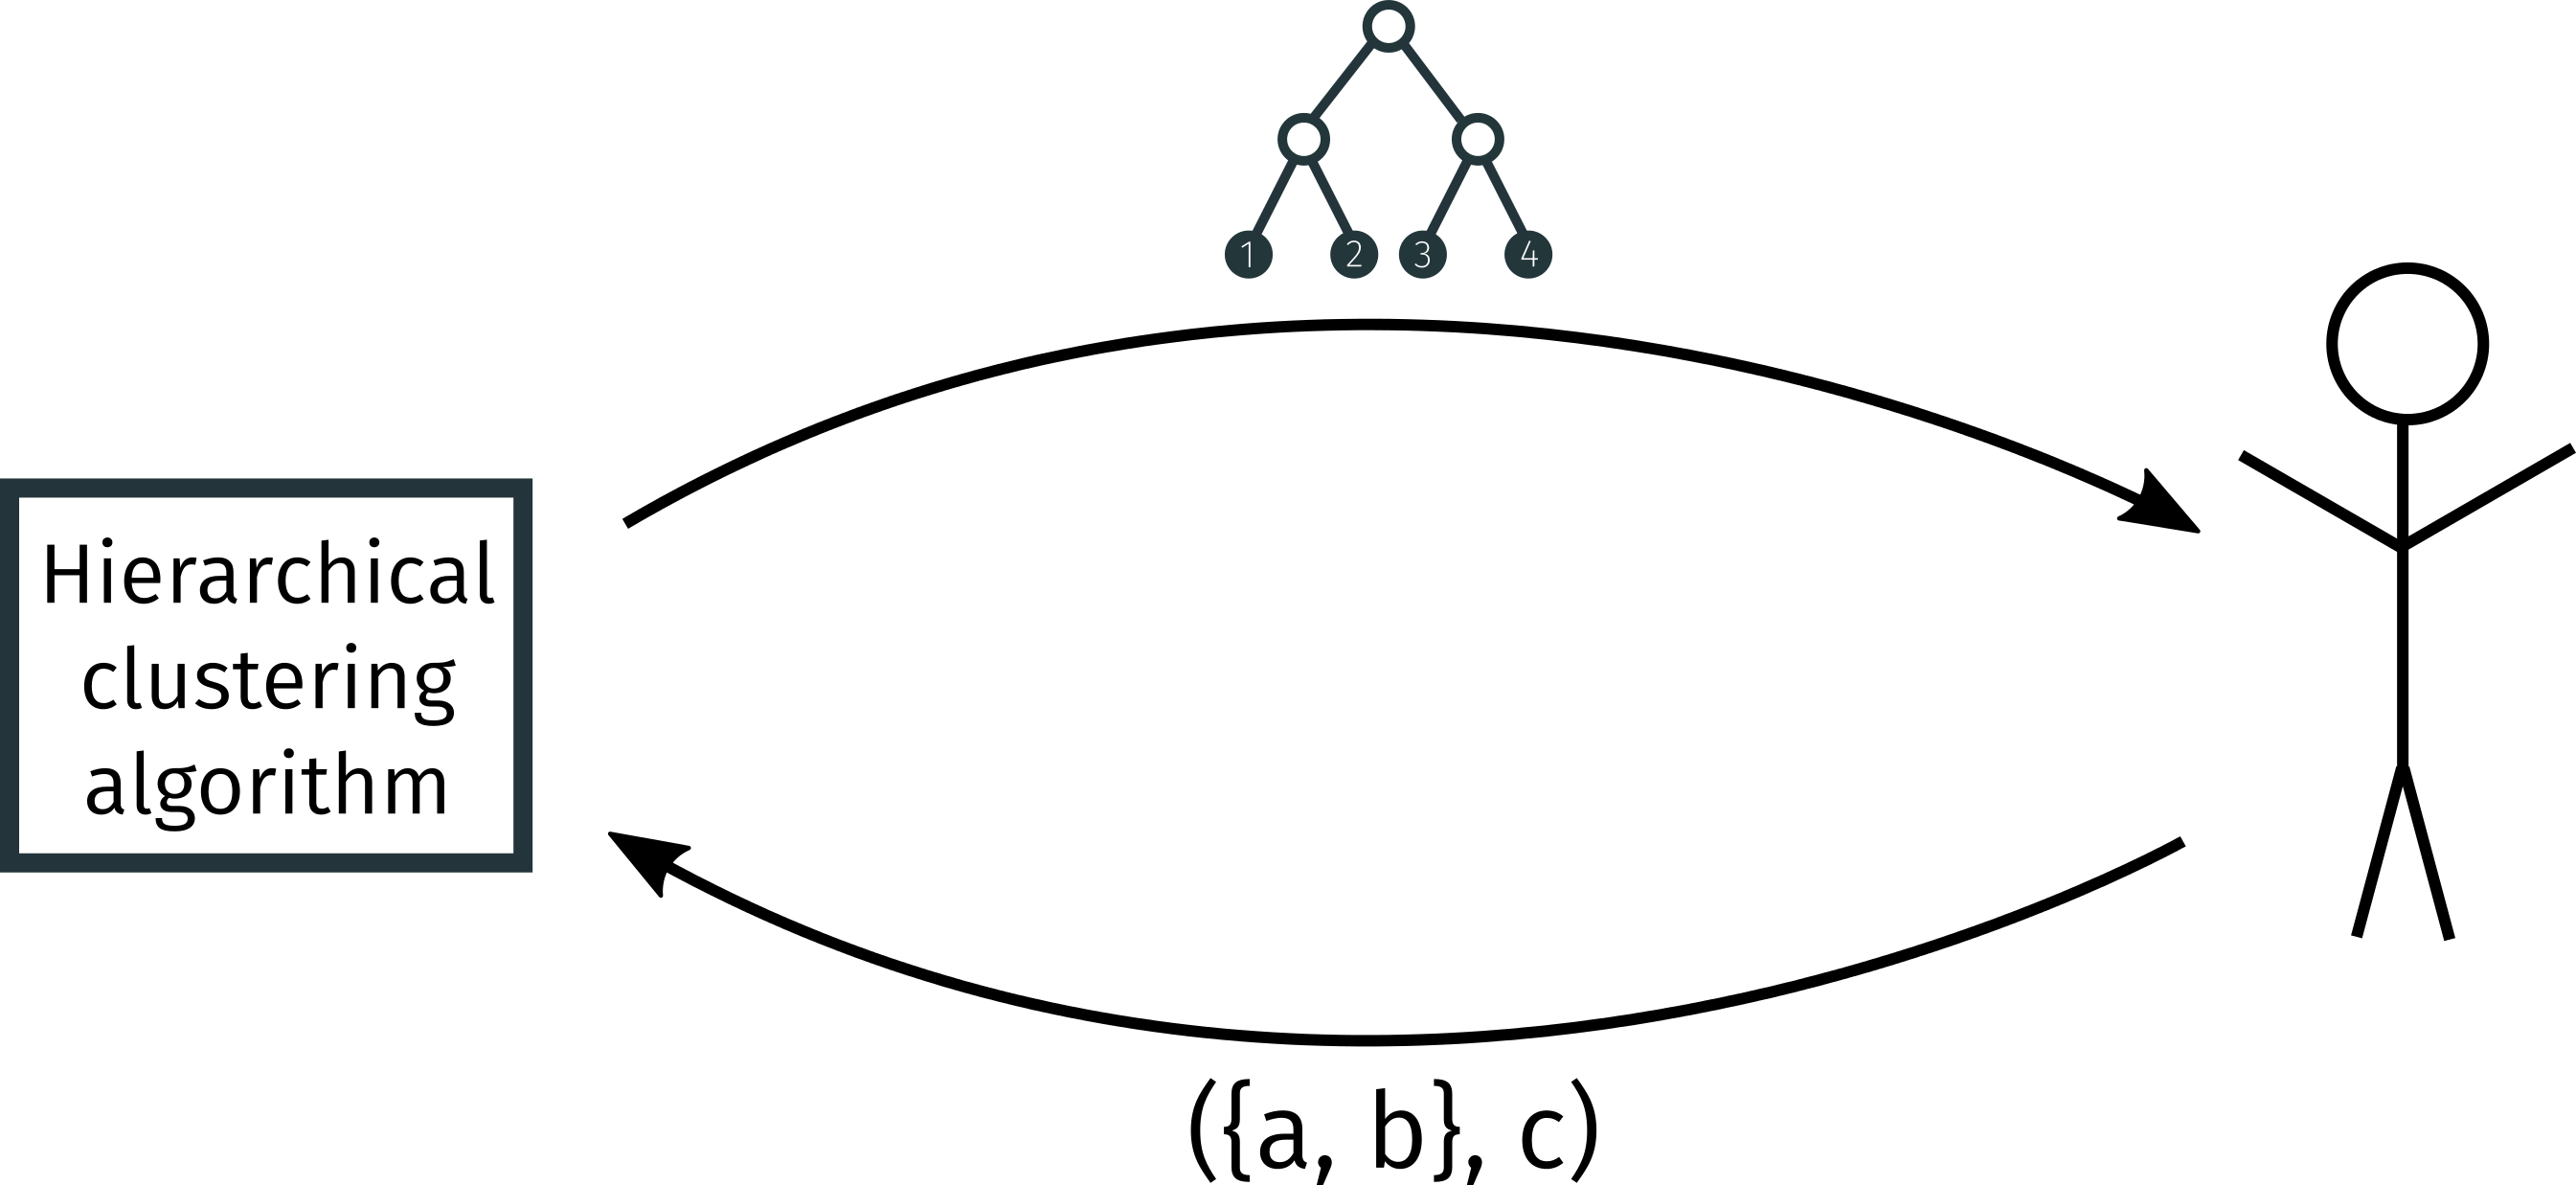
\includegraphics[width=0.7\textwidth]{img/interaction-3}
  \end{center}
  \pause

  \textbf{Idea:}  enforce triplet constraints with
  modified SPR move

  \pause

  \begin{center}
    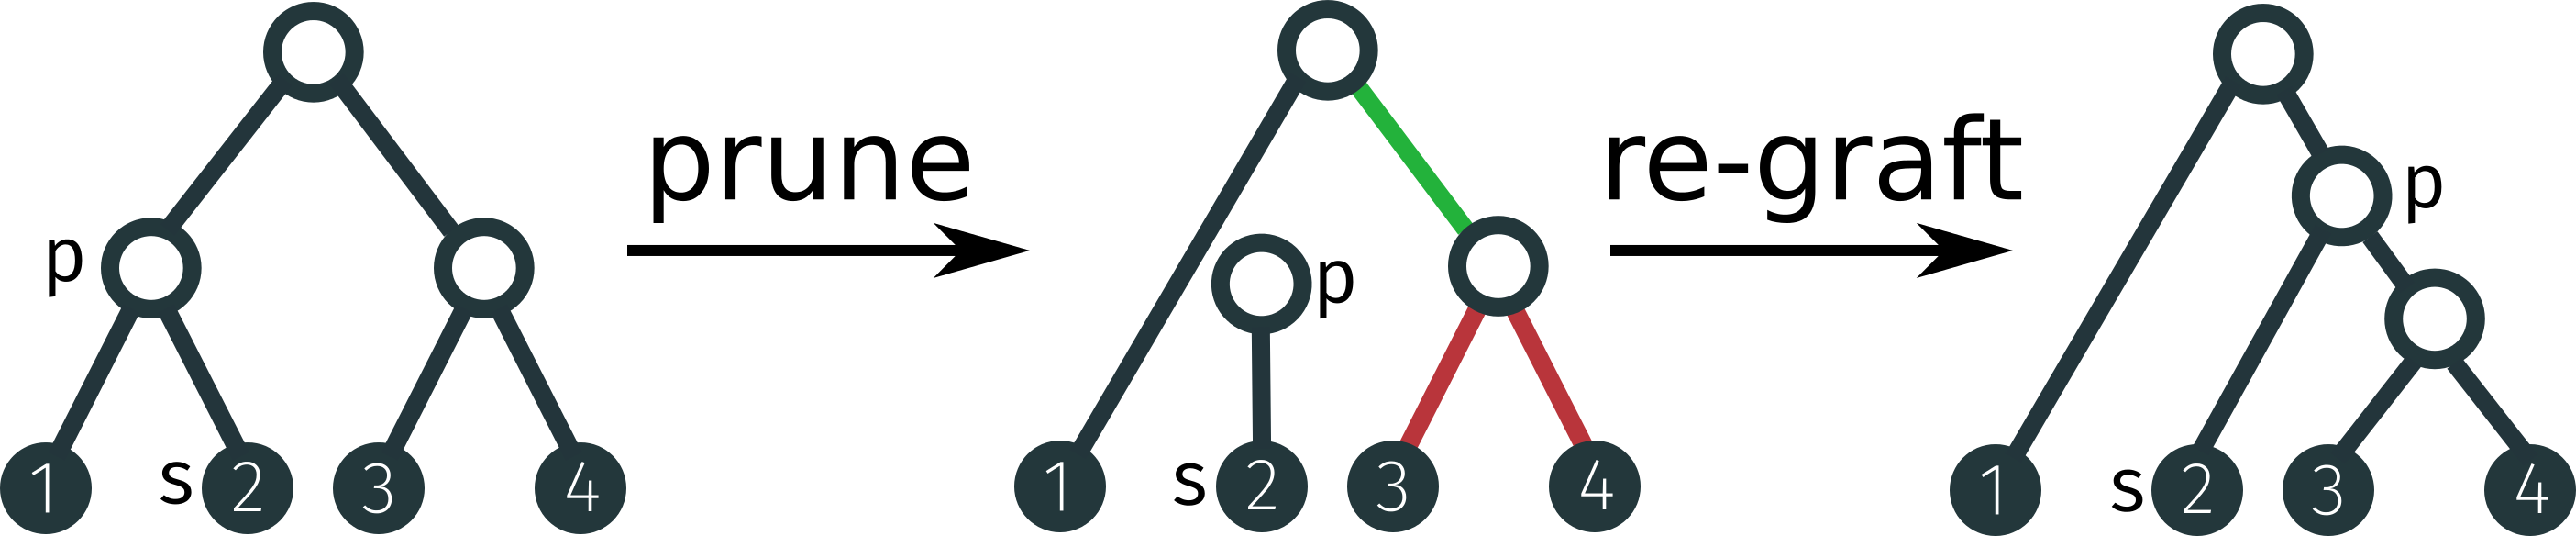
\includegraphics[width=\textwidth]{img/cspr-animation}
  \end{center}
\end{frame}

\begin{frame}{Intelligent subset queries}

  Recall the interaction model.

  \begin{center}
    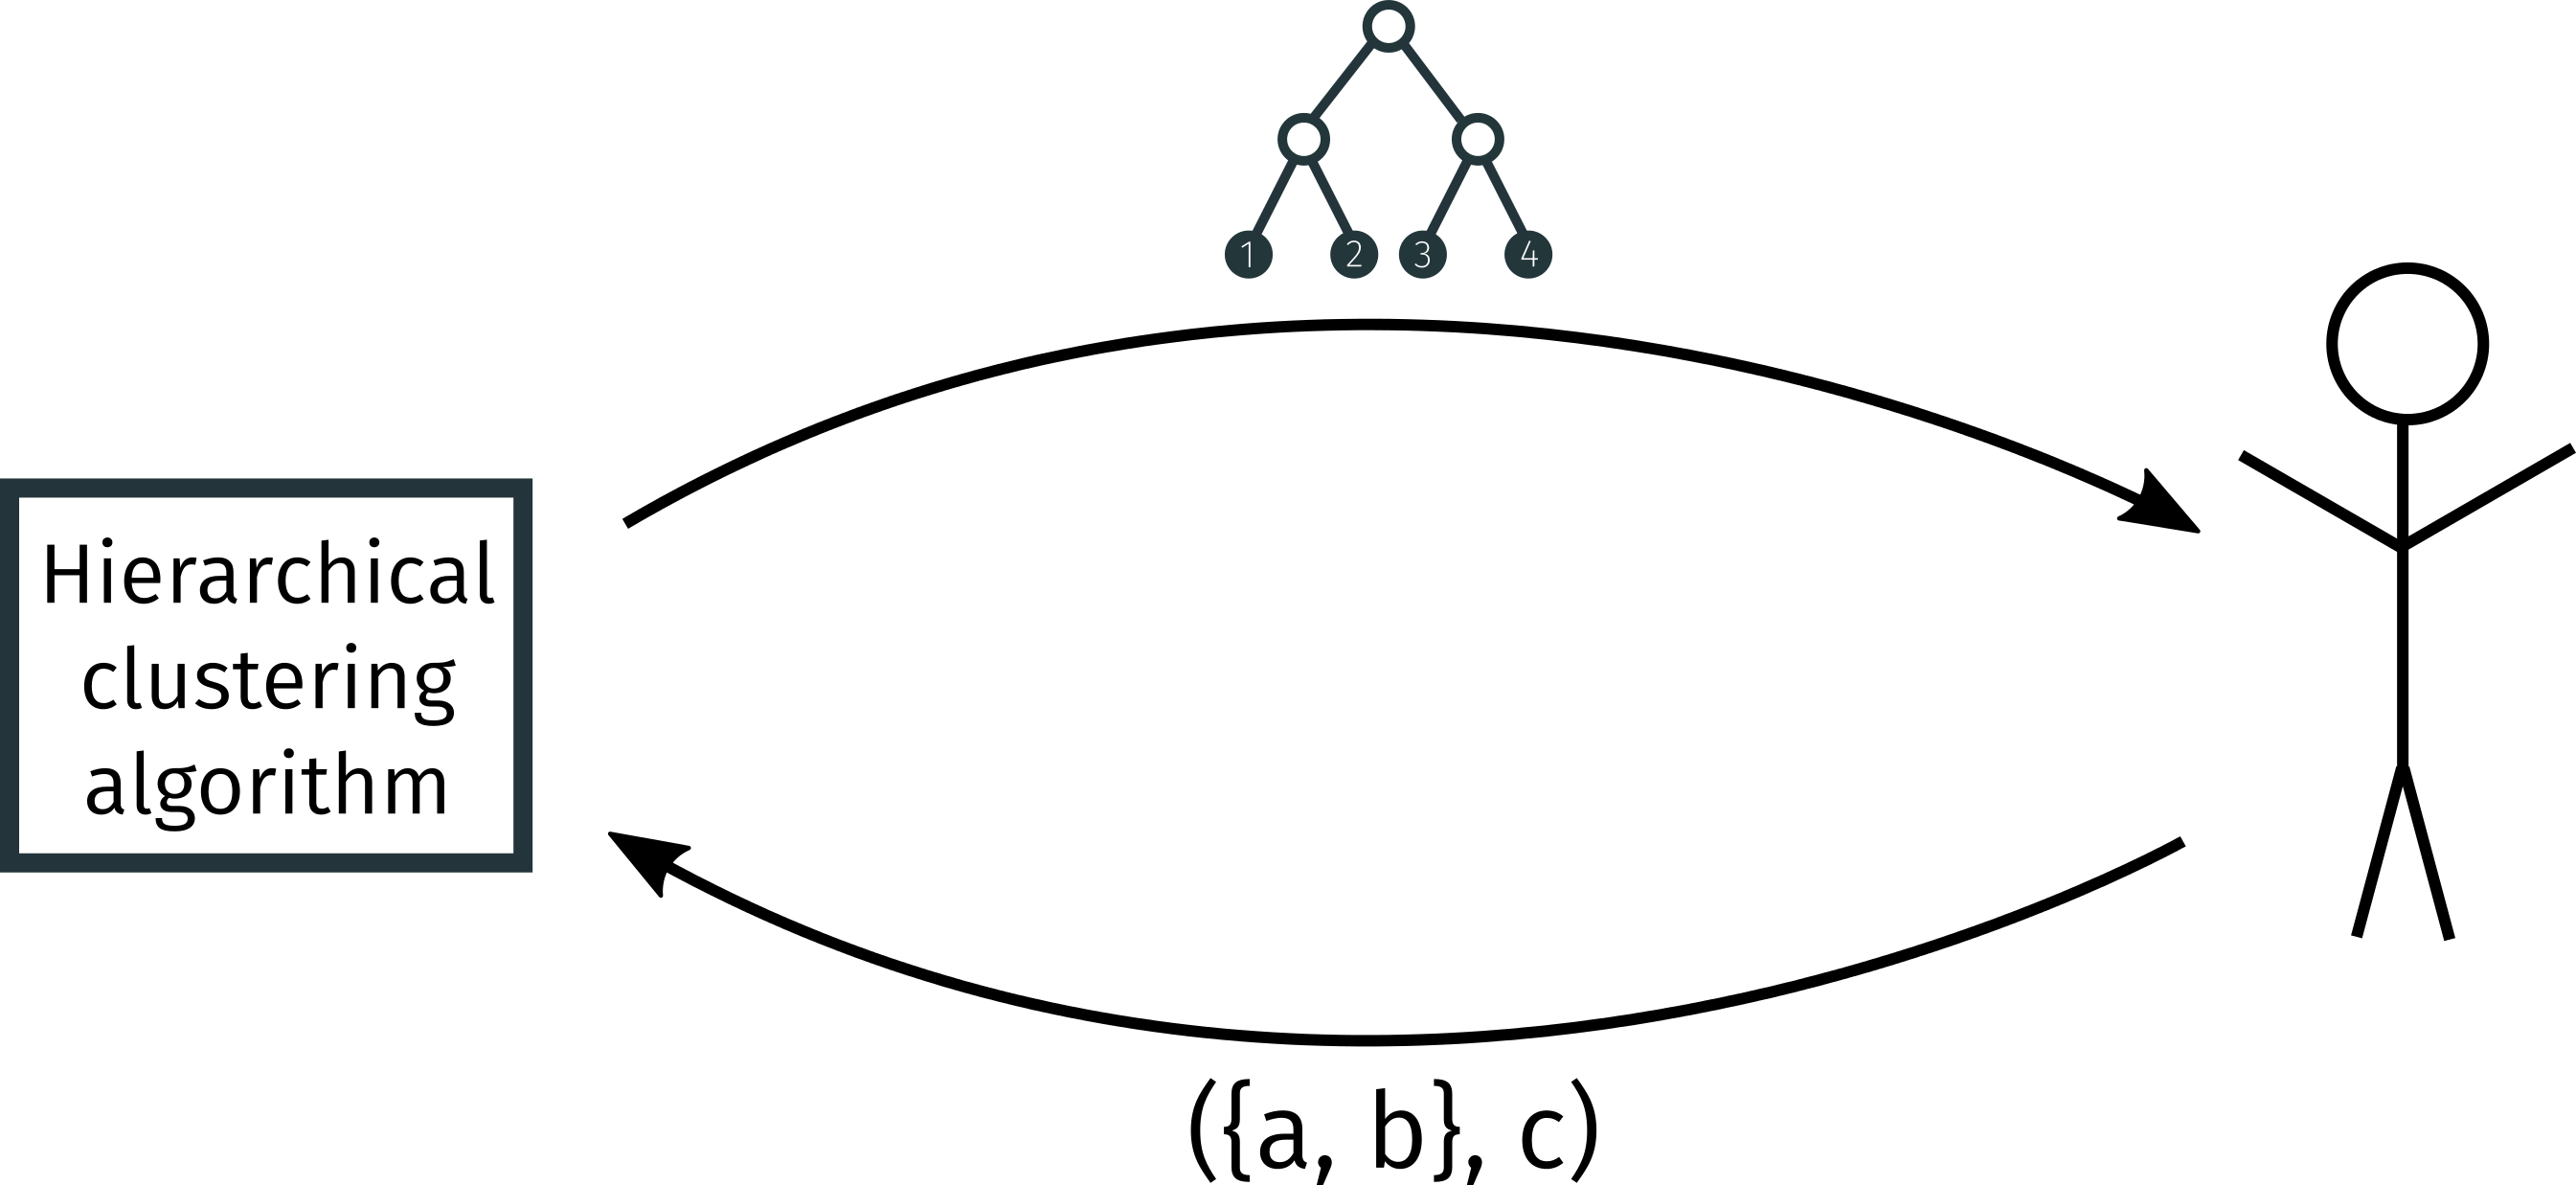
\includegraphics[width=\textwidth]{img/interaction-3}
  \end{center}

  \pause

  %We pick a subset of data $S$ and show a user the candidate tree
  %restricted to $S$, $T|_S$.

  %\pause

  \textbf{Idea:}  pick subsets that have high variance
  under the posterior distribution

\end{frame}

\begin{frame}{Measuring subtree variance}

    First, sample $N$ trees from posterior distribution.

  \pause

 \metroset{block=fill}
  \begin{block}{Definition: tree distance variance (TDV)}
    Given a subset of data $S$ and tree samples $\mathcal{T} = T_1, \ldots, T_N$,
    \begin{align}
      \mathrm{TDV}(S, \mathcal{T}) = \max_{i, j \in S}  \mathrm{Var}_{T \in \mathcal{T}}\left[\texttt{tree-dist}_{T|S}(i, j)\right]
    \end{align}
  where $\texttt{tree-dist}_T$ is the number of edges needed to get from leaf $i$ to leaf $j$
  in tree $T$.
  \end{block}

  \pause

Instantiate $L$ subsets randomly and pick the one with the highest variance.

\end{frame}

\begin{frame}{Evaluation}
  We evaluate 5 different querying schemes.
  \begin{itemize}
    \item<2-> \textbf{Simple:} 3 leaves chosen at random.
    \item<3-> \textbf{Random:} Induced subtree of a random subset.
    \item<4-> \textbf{Active:} Induced subtree of high variance subset.
    \item<5-> \textbf{Interleaved:} Alternatively random and active
    \item<6-> \textbf{Smart:} Entire candidate tree
  \end{itemize}

  \uncover<7->{
  We used the Dirichlet diffusion tree prior,
  running samplers for 60000 iterations, issuing
  queries every 100 iterations.
  }

  \uncover<8->{
 \metroset{block=fill}
  \begin{block}{Definition: triplet distance (TD)}
    Given a tree $T$ and a ground truth tree $T^*$,
    \begin{align}
      \mathrm{TD}(T^*, T) = \frac{\sum_{c \in \Delta(T^*)} \mathbb{I}(c \notin \Delta(T)) }{|\Delta(T^*)|}
    \end{align}
  where $\Delta(T)$ is the set of all proper triplet constraints embodied
  in tree $T$.
  \end{block}
}
\end{frame}

\begin{frame}{Experiments}
\begin{figure}
    \centering
    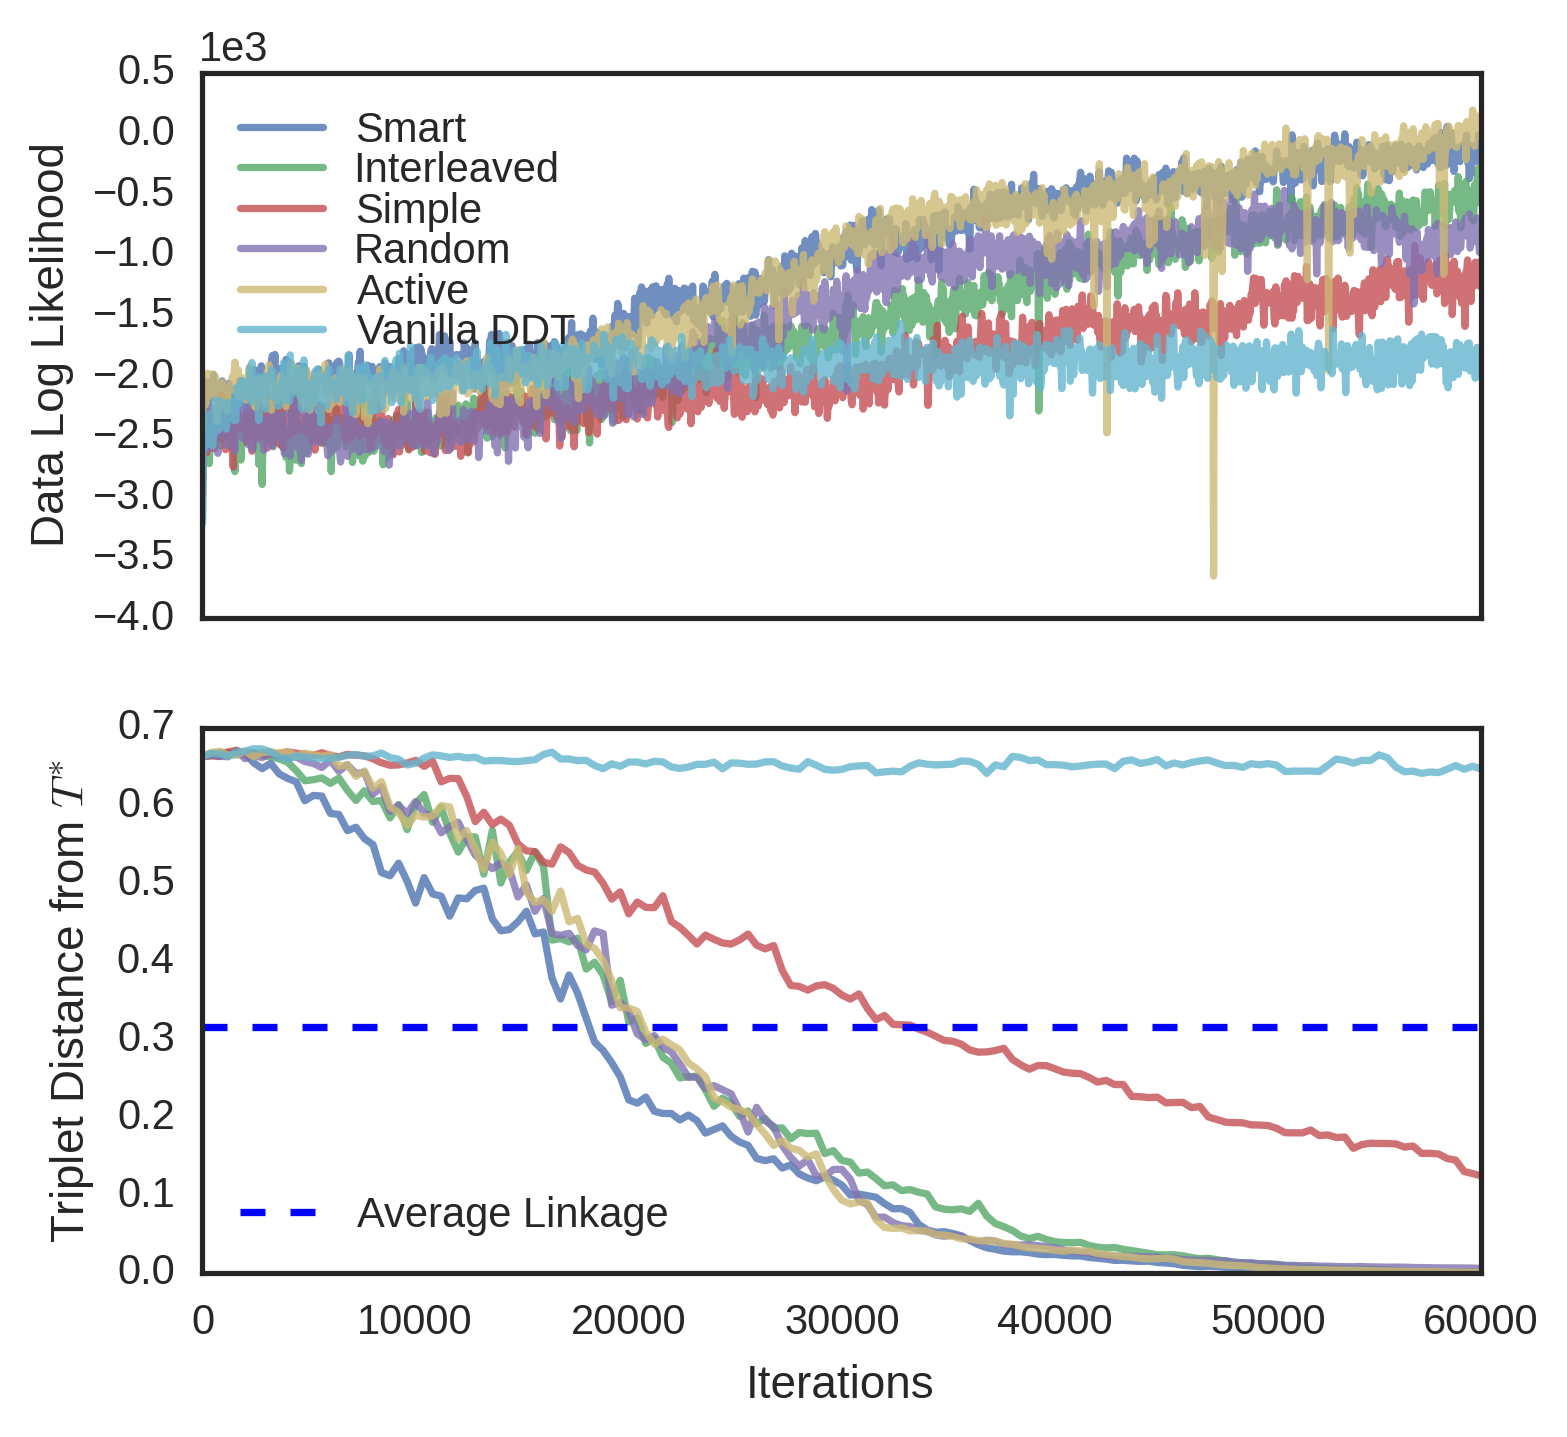
\includegraphics[frame, width=0.7\textwidth]{img/interactive}
    \caption{\emph{Zoo} dataset}
    \label{fig:ibhc}
  \end{figure}
\end{frame}

\begin{frame}{Experiments}
\begin{figure}
    \centering
    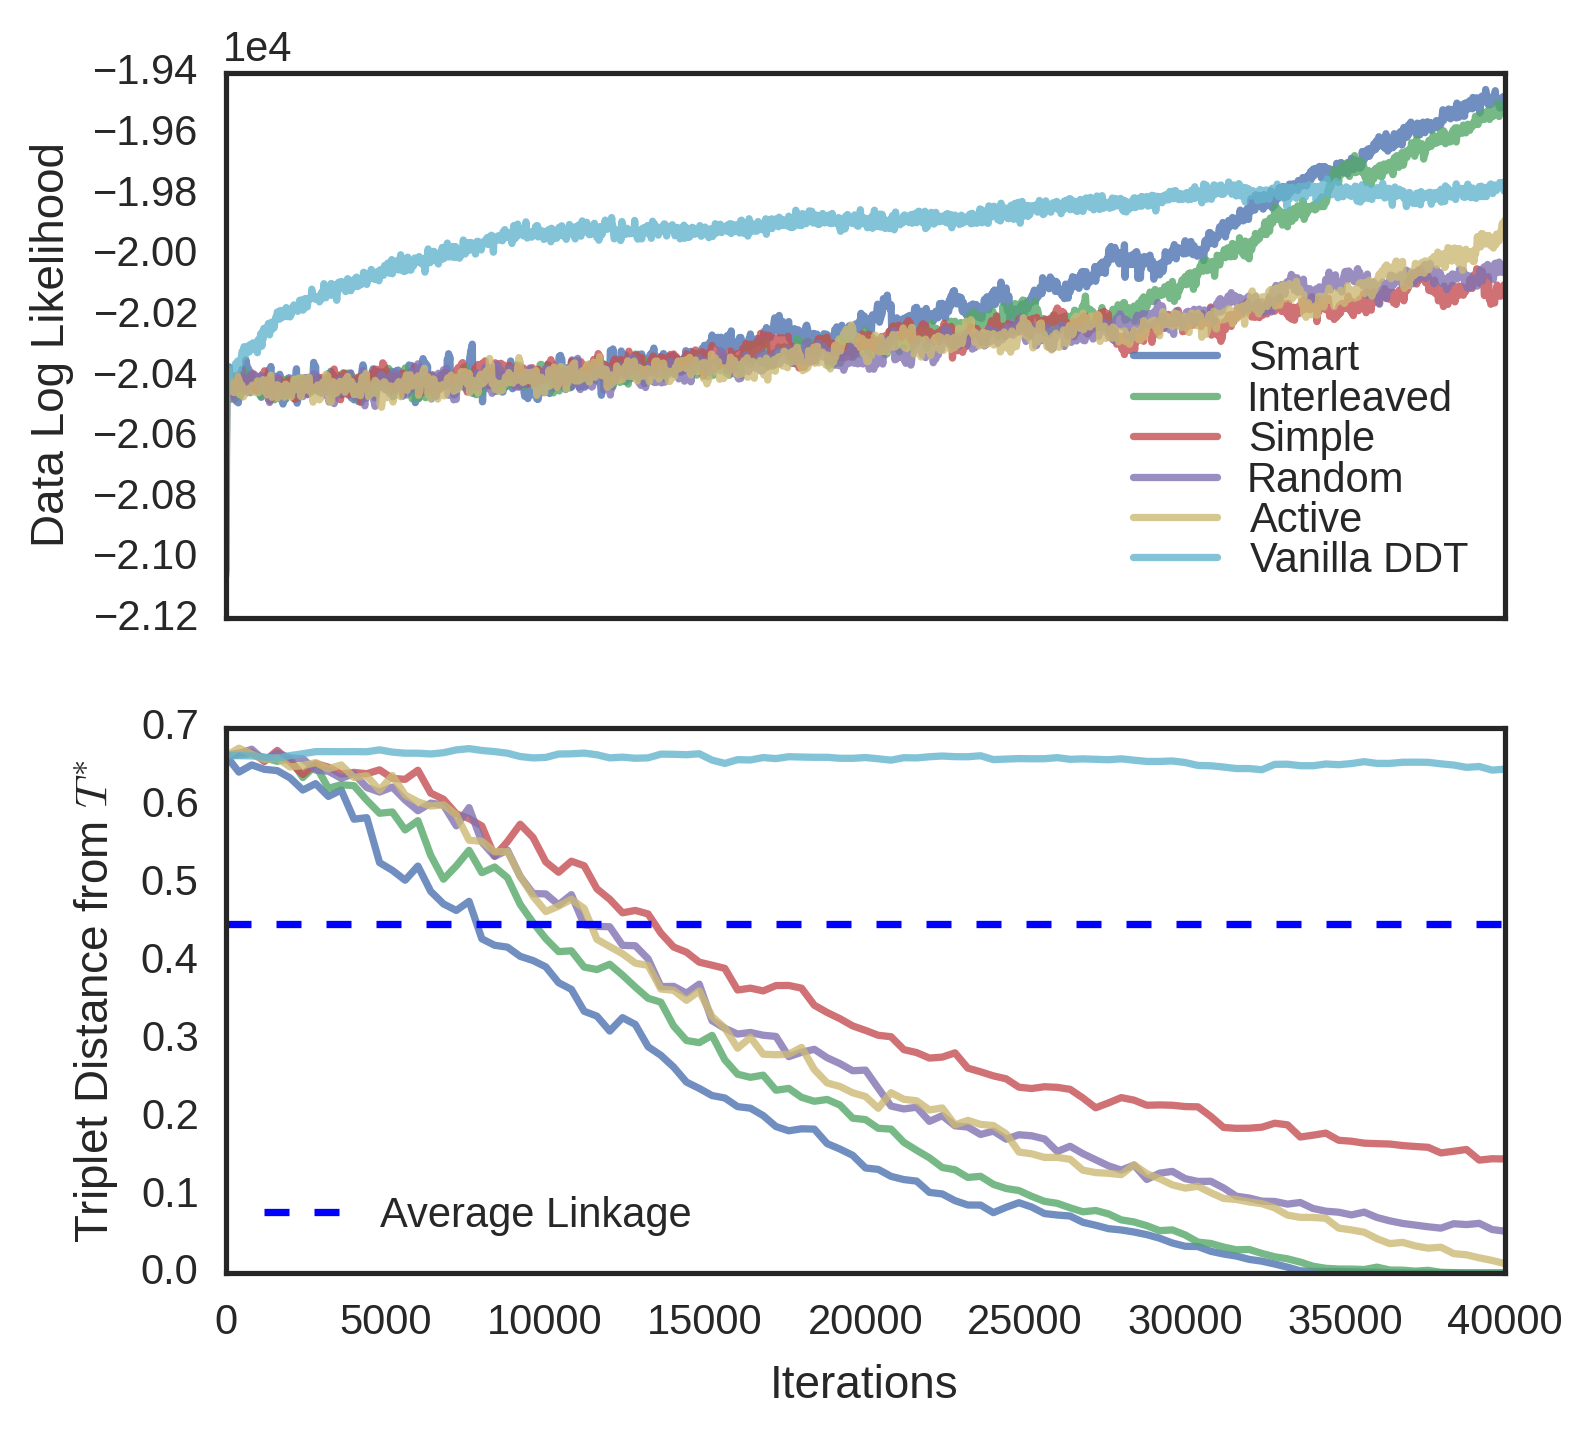
\includegraphics[frame, width=0.7\textwidth]{img/interactive-2}
    \caption{\emph{MNIST} dataset}
    \label{fig:ibhc}
  \end{figure}
\end{frame}

\begin{frame}{Experiments}
\begin{figure}
    \centering
    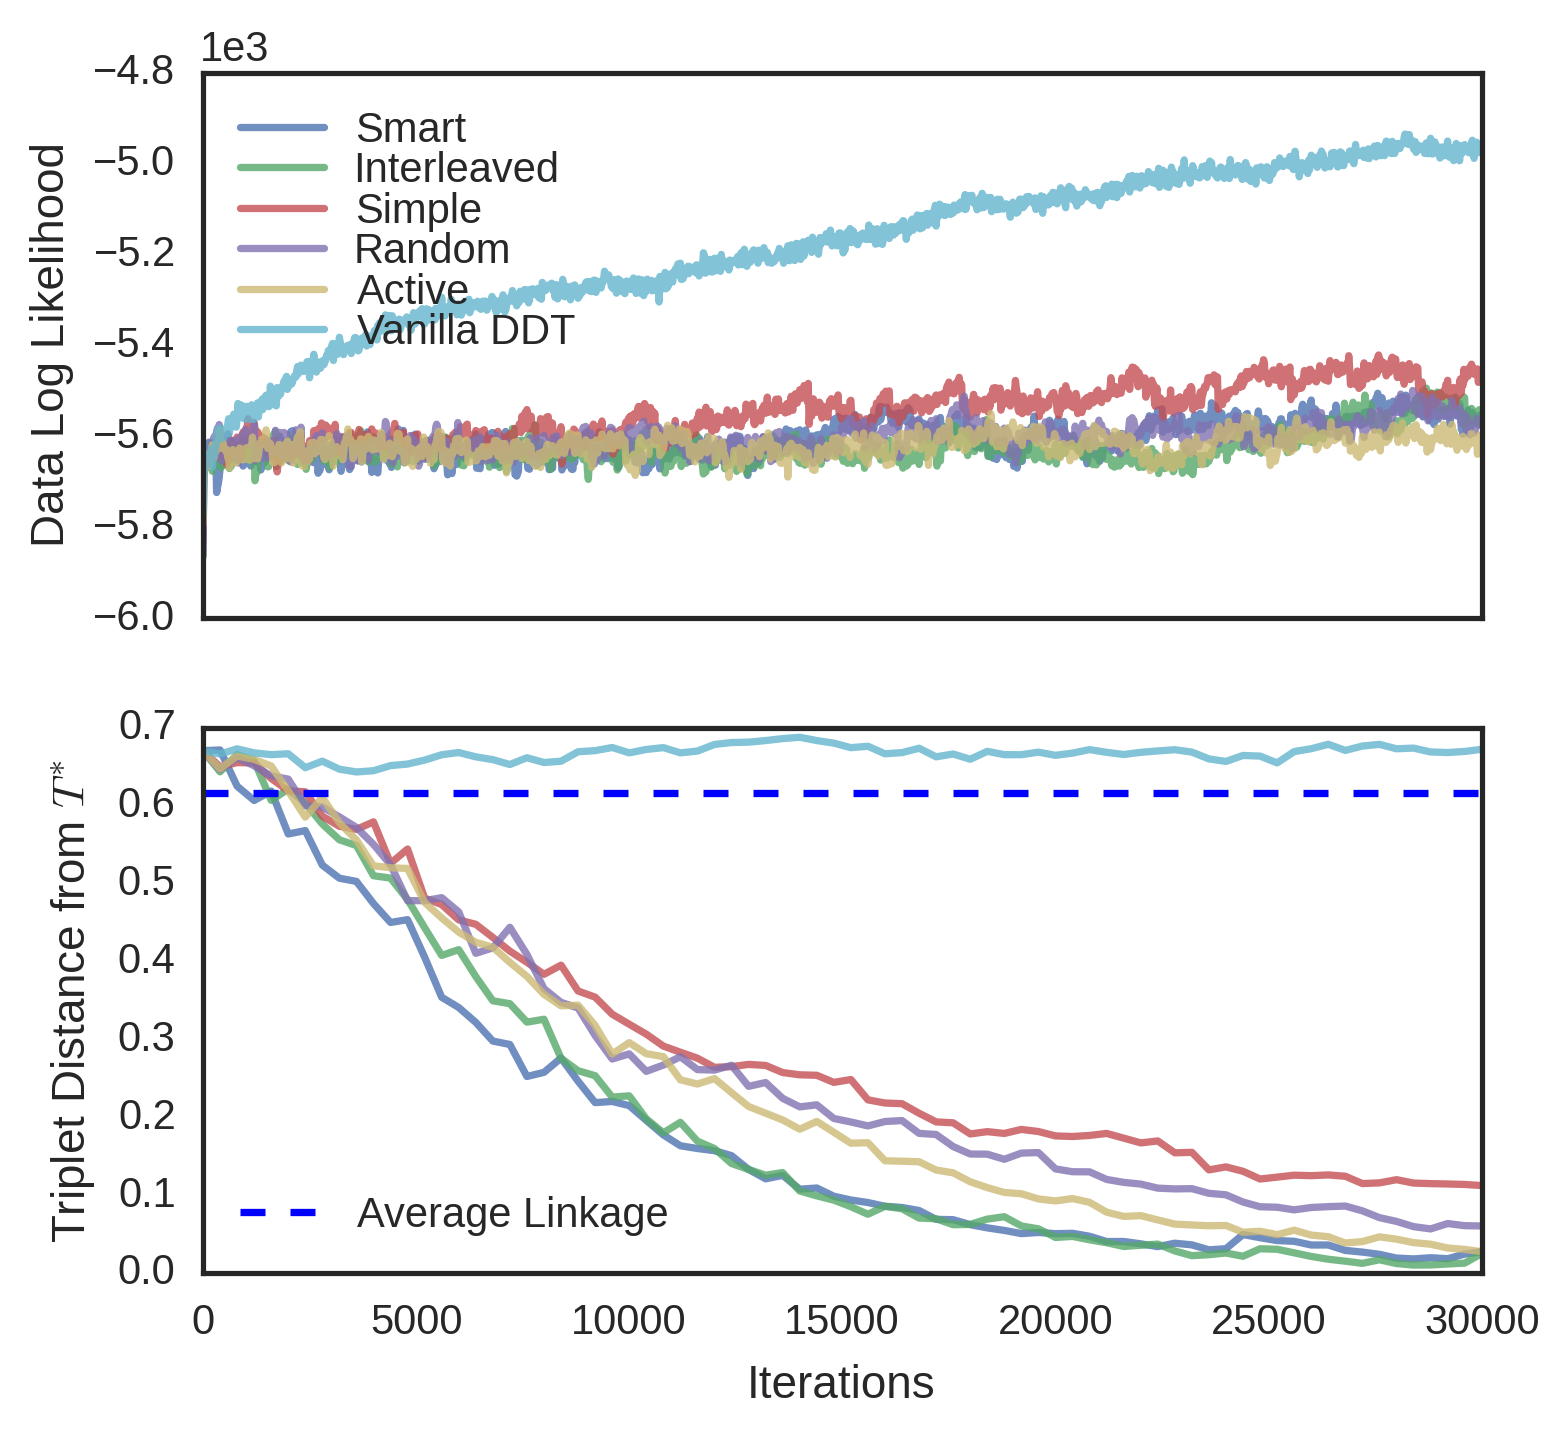
\includegraphics[frame, width=0.7\textwidth]{img/interactive-3}
    \caption{\emph{20 Newsgroups} dataset}
    \label{fig:ibhc}
  \end{figure}
\end{frame}

\begin{frame}[standout]
Thank you!
\end{frame}

%\begin{frame}{Metropolis-Hastings}
  
  %The \alert{Metropolis-Hastings} (MH) algorithm
  %is an MCMC method that uses
  %samples from a distribution $p(x)$ to approximate it.

  %\pause
 %\metroset{block=fill}
  %\begin{block}{Metropolis-Hastings algorithm}
    %\begin{itemize}
      %\item Given initial distribution $p_0(x)$ and proposal distribution
        %$q(x'|x)$
      %\item Instantiate $x_0$ by sampling $p_0(x)$.
      %\item Repeat for $t = 1 \ldots T$
        %\begin{itemize}
          %\item Sample $x'$ from $q(x'|x_{t - 1})$.
          %\item Calculate acceptance ratio
            %\begin{align}
                %\alpha = \frac{p(x')q(x_t | x')}{p(x_t)q(x' | x_t)}
            %\end{align}
          %\item If $\alpha > 1$, accept the sample, setting $x_t = x'$
          %\item If $\alpha \le 1$, accept $x'$ with probability $\alpha$
            %and reject otherwise, setting $x_t = x_{t - 1}$.
        %\end{itemize}
    %\end{itemize}
  %\end{block}
%\end{frame}

%\begin{frame}{Ambiguous data}
  %Consider the two following scenarios where
  %circles represent tight clusters of data.

  %\begin{center}
  %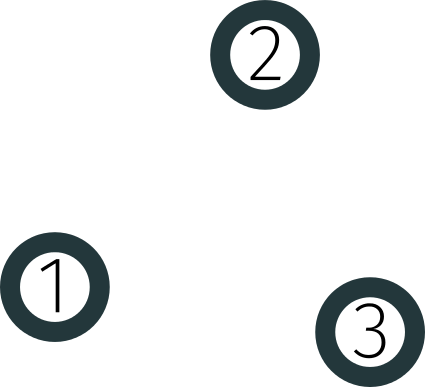
\includegraphics[width=0.3\textwidth]{img/3-cluster}\hfill
  %\includegraphics[width=0.45\textwidth]{img/3-cluster-line}
  %\end{center}

  %\pause

  %A single binary tree is not sufficient to describe either
  %of these configurations.

  %%\centering
  %%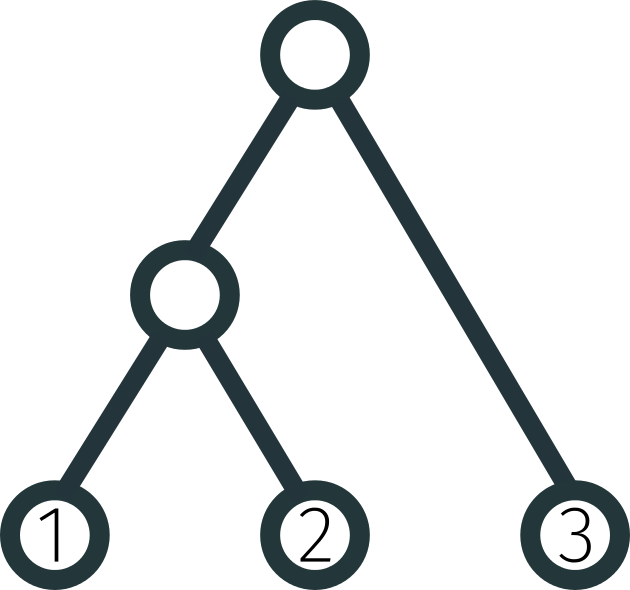
\includegraphics[width=0.3\textwidth]{img/tree-123} \hfill
  %%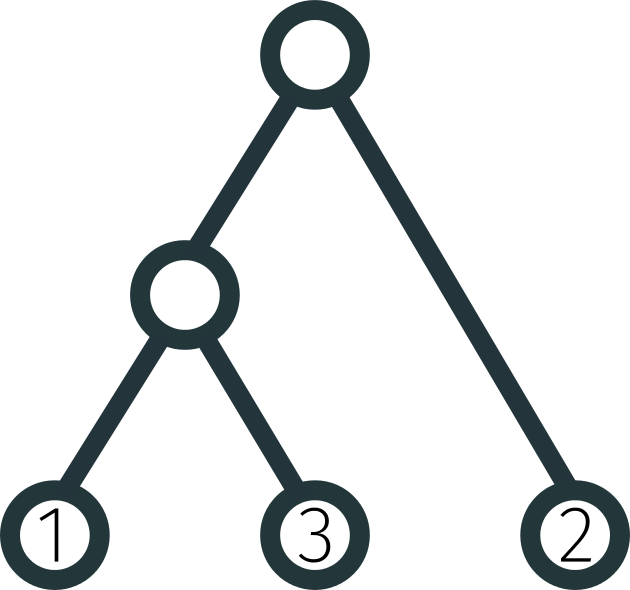
\includegraphics[width=0.3\textwidth]{img/tree-132} \hfill
  %%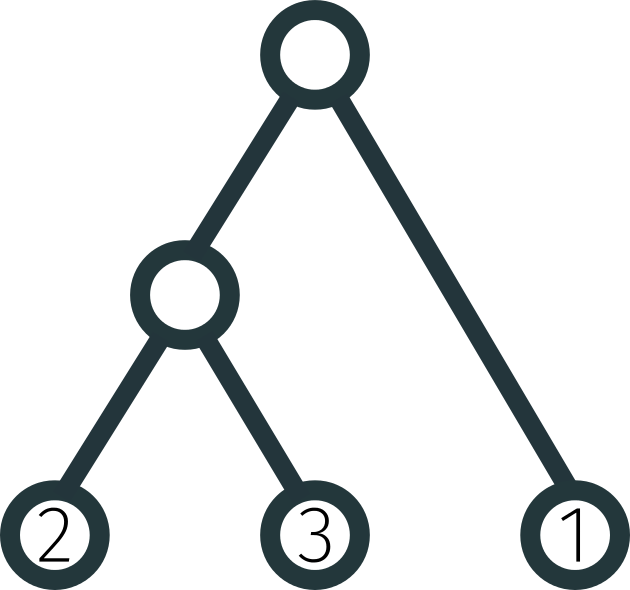
\includegraphics[width=0.3\textwidth]{img/tree-231}

%\end{frame}

%\begin{frame}{Multifurcating trees}
  %Perhaps extending our binary trees to $k$-ary trees will help.

  %\begin{center}
    %\includegraphics<1>[width=0.8\textwidth]{img/3-cluster-both.png}
    %\includegraphics<2>[width=0.8\textwidth]{img/3-cluster-both-2.png}
    %\includegraphics<3>[width=0.8\textwidth]{img/3-cluster-both-3.png}
  %\end{center}

%\end{frame}

%\begin{frame}{Uncertainty in hierarchies}
  %Furthermore, small perturbations in our data
  %can have an effect on the output
  %hierarchy.

  %\begin{center}
    %\includegraphics<1>[width=0.8\textwidth]{img/3-cluster-line-noperturb}
    %\includegraphics<2->[width=0.8\textwidth]{img/3-cluster-line-perturb}
  %\end{center}

  %%\uncover<3>{We need a more general approach.}
%\end{frame}

%\begin{frame}{Probabilistic reasoning}
  %One approach is to
  %model ambiguity and uncertainty with \textbf{probability}.
  %We output a probability distribution over all possible
  %trees.

  %\begin{center}
    %\includegraphics<2>[width=0.7\textwidth]{img/3-cluster-distribution.png}
    %\includegraphics<3>[width=0.7\textwidth]{img/3-cluster-linear-distribution.png}
  %\end{center}
%\end{frame}

%\subsection{Bayesian learning}

%\begin{frame}{Latent variable models}
  %We take a quick detour to review Bayesian learning.
  %\begin{center}
    %\includegraphics<2>[width=0.1\textwidth]{img/latent-variable-model-0}
    %\includegraphics<3->[width=0.1\textwidth]{img/latent-variable-model}
  %\end{center}
%\uncover<4->{
  %Our data $X$ is generated conditionally given a set of
  %unobserved \alert{latent} variables $\theta$.
%}
%\end{frame}

%\begin{frame}{Distributions of interest}
  %We are interested in the \alert{posterior distribution}
  %of latent variables given data, $P(\theta | X)$,
  %calculated via Bayes rule.
  %\pause

  %\begin{align}
    %P(\theta | X) = \frac{P(X | \theta)P(\theta)}{P(X)} = \frac{P(X | \theta)P(\theta)}{\int_\Theta P(X|\theta)P(\theta)d\theta}
  %\end{align}
  %\pause
  %$P(\theta)$ is called the \alert{prior distribution} and $P(X|\theta)$ is called the
  %\alert{likelihood model}. They are specified beforehand.
%\end{frame}

%\begin{frame}{Bayesian inference}
  %Typically the hardest part of computing the
  %the posterior distribution is calculating
  %$P(X) = \int_\Theta P(X|\theta)P(\theta)d\theta$, the \alert{marginal distribution}.

   %\pause 

  %When the prior $P(\theta)$ and likelihood $P(X|\theta)$ are
  %conjugate, the posterior is analytically computable.

  %\pause

  %Otherwise, we usually approximate it with methods such as:
  %\begin{itemize}
    %%\item Loopy belief propagation
    %\item Markov chain Monte Carlo (MCMC)
    %\item Variational inference
    %\item MAP estimation via EM
  %\end{itemize}
%\end{frame}

%\section{Bayesian hierarchical clustering}

%\begin{frame}{BHC as a latent variable model}
  %Bayesian hierarchical clustering is a
  %statistical approach, specifically
  %a \alert{latent variable model}.
  %\pause
  %\begin{center}
    %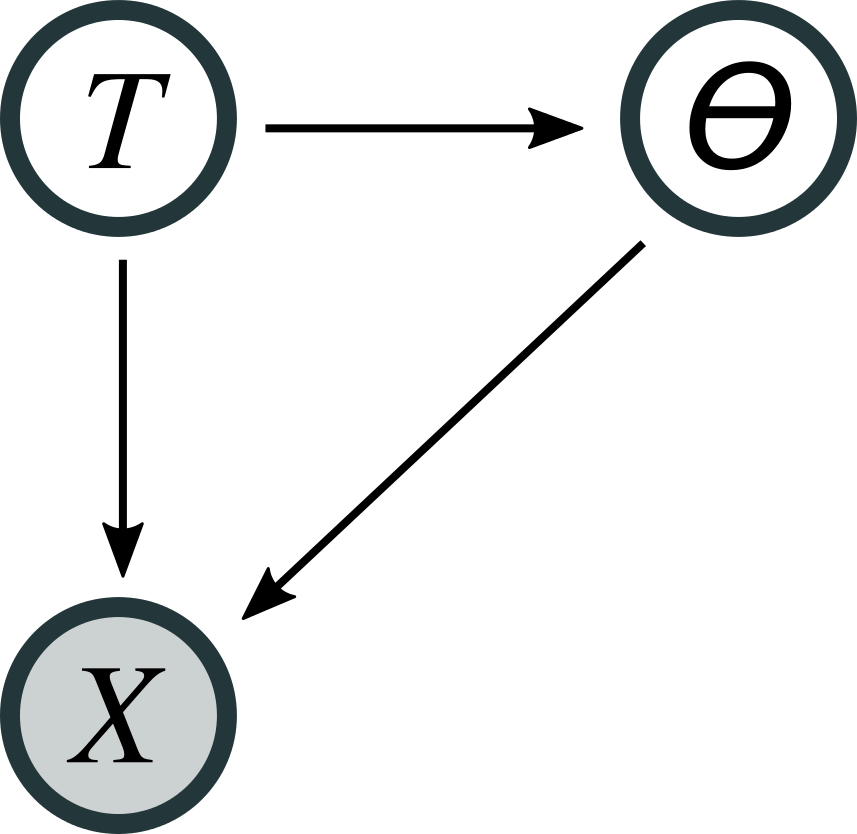
\includegraphics[width=0.3\textwidth]{img/bhc-lvm}
  %\end{center}
  %It is composed of data $X$ and
  %latent variables $T$ and $\theta$.
  %\pause
  %\begin{itemize}
    %\item $T$ is a tree structure, sampled from a \alert{tree prior} distribution $P(T)$.
    %\item $\theta$ is a set of parameters, generated in a \alert{tree likelihood} model $P(\theta | T)$.
  %\end{itemize}
%\end{frame}

%\begin{frame}{Tree priors}
  %Most often we are interested in rooted binary trees with labeled leaves,
  %also called \alert{cladograms}.

  %\begin{center}
    %\includegraphics<1>[width=0.4\textwidth]{img/tree-4}
    %\includegraphics<2>[width=0.4\textwidth]{img/tree-4-ordering}
    %\includegraphics<3>[width=0.4\textwidth]{img/tree-4-ordering-times}
  %\end{center}

  %Very often, cladograms will contain additional information.

  %\begin{itemize}
    %\item<2-> An ordering on the internal nodes
    %\item<3-> Times associated with each node
  %\end{itemize}

%\end{frame}

%\begin{frame}{Tree priors}
  %The simplest tree prior is the uniform distribution over
  %cladograms.

  %\pause

  %\begin{center}
    %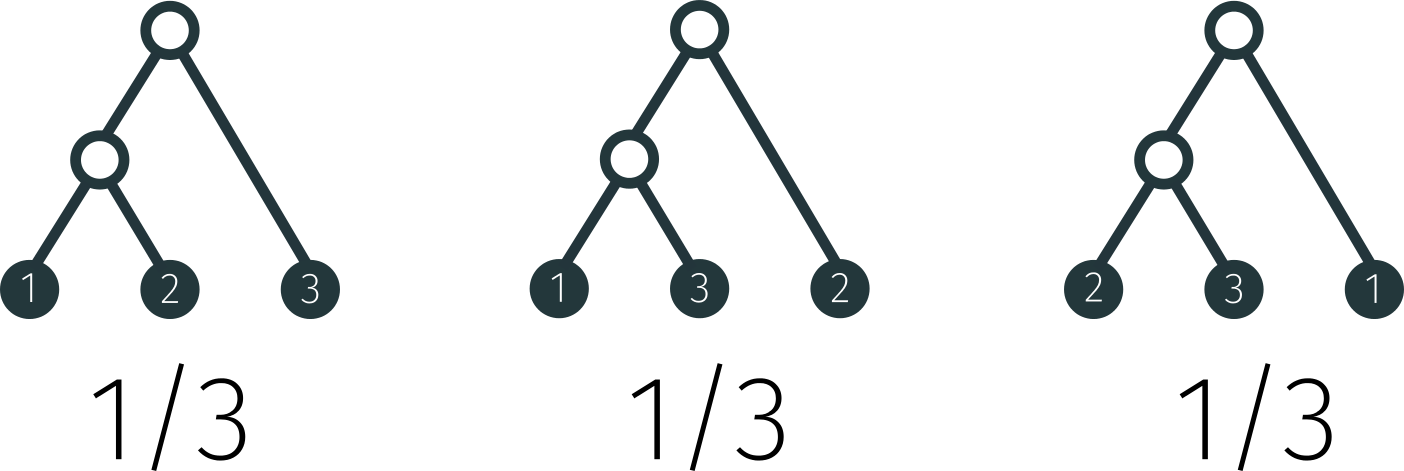
\includegraphics[width=0.6\textwidth]{img/uniform-distribution}
  %\end{center}

  %\pause

  %Tree priors mostly fall into two categories:
  %\pause
 %\metroset{block=fill}
  %\begin{block}{Coalescent models}
    %Trees are modeled in an
      %agglomerative fashion, merging clusters until 
      %one is left
    %\end{block}
  %\pause
  %\begin{block}{Diffusion models}
    %Trees are modeled inductively,
      %starting with a tree of size $1$ and growing it to
      %a tree of size $N$.
    %\end{block}
%\end{frame}

%\subsection{Coalescent models}

%\begin{frame}{Coalescent models}
  %Coalescent models begin with a set of $N$
  %data, or "individuals", at $t = 0$.

  %\begin{center}
    %\includegraphics<1>[width=0.5\textwidth]{img/coalescent-1}
    %\includegraphics<2>[width=0.5\textwidth]{img/coalescent-2}
    %\includegraphics<3>[width=0.5\textwidth]{img/coalescent-3}
    %\includegraphics<4>[width=0.5\textwidth]{img/coalescent-4}
  %\end{center}

  %\pause

  %Every iteration, we:
  %\begin{itemize}
    %\item Pick two distinct nodes $a$ and $b$ uniformly at random.
    %\item Sample a coalesce time $t$.
    %\item Create an internal node whose children are $a$ and $b$
      %with time $t$.
  %\end{itemize}
%\end{frame}


%\begin{frame}{Kingman's coalescent}
  %The canonical coalescent model is \alert{Kingman's coalescent} \cite{Kingman1982}.

  %There are a total of
  %$N - 1$ events happening at time $t_{N - 1} < t_{N - 2} < \cdots < t_1$,
  %which happen at a constant coalesce rate.

  %\pause

  %\begin{center}
    %
\includegraphics[width=\textwidth]{img/coalescent-times}
  %\end{center}

  %\pause


    %Let $\delta_i$ represent the elapsed time
  %between coalescent event $i-1$ and $i$.
  %We let
  %\begin{align}
    %\delta_i \sim \mathrm{Exp}\left(\binom{N - i + 1}{2}\right)
  %\end{align}

%\end{frame}

%\begin{frame}{Kingman's coalescent}
  %\begin{itemize}
    %\item<1-> Kingman's coalescent corresponds
  %to the uniform distribution
  %over \emph{ordered cladograms}.

    %\item<2-> Its induced distribution over
  %unordered cladograms is the time-marginalized coalescent (TMC) \cite{Boyles2012}.

    %\item<3-> What sort of trees does Kingman's coalescent favor?
      %\begin{center}
        %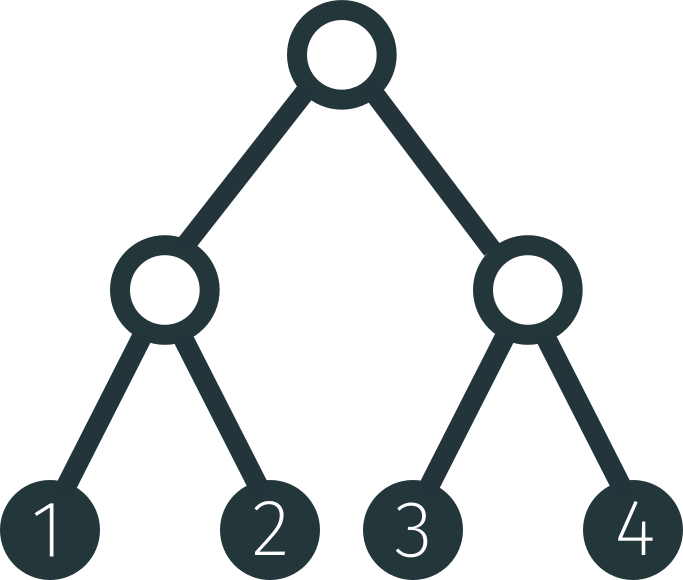
\includegraphics[width=0.4\textwidth]{img/tree-1234-balanced} \hspace{0.4em}
        %\includegraphics[width=0.37\textwidth]{img/tree-4-unbalanced}
      %\end{center}
  %\end{itemize}
%\end{frame}


%\subsection{Diffusion models}

%\begin{frame}{Diffusion models}
  %Basic idea: begin with a tree over
    %one data, then for $N$ iterations:
  %\begin{itemize}
    %\item Sample a branch and time at random.
    %\item Attach a leaf to the branch,
      %creating a new internal node with the sampled time.
  %\end{itemize}
  %\begin{center}
    %\includegraphics<2>[width=\textwidth]{img/diffusion-1}
    %\includegraphics<3>[width=\textwidth]{img/diffusion-2}
    %\includegraphics<4>[width=\textwidth]{img/diffusion-3}
    %\includegraphics<5>[width=\textwidth]{img/diffusion-4}
  %\end{center}
%\end{frame}

%\begin{frame}{Dirichlet diffusion tree}
    %The simplest model is the Dirichlet diffusion tree (DDT),
    %which produces trees with both ordering
    %and times associated with internal nodes \cite{Neal2003}.

    %The model is defined inductively via a continuous time
    %process. Assume we have a tree of size $i - 1$.

    %\pause

    %\begin{center}
      %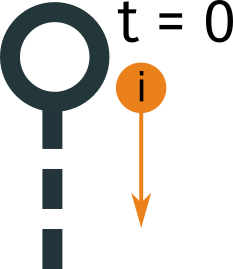
\includegraphics[width=0.2\textwidth]{img/ddt-1}
    %\end{center}

    %On each iteration, a particle labeled $i$ begins at the root and travels downwards.
%\end{frame}

%\begin{frame}{Dirichlet diffusion tree}
  %\textbf{Case 1:} 
  %The particle reaches an internal node.
  %\begin{center}
      %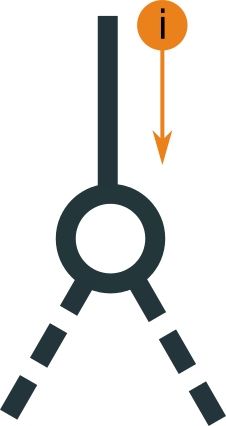
\includegraphics[width=0.13\textwidth]{img/ddt-2}
  %\end{center}

  %\pause

  %It picks one of the branches proportional to the past number
  %of particles that have picked either branch.

  %\pause

  %\begin{center}
      %\includegraphics[width=0.17\textwidth]{img/ddt-3}
  %\end{center}
%\end{frame}

%\begin{frame}{Dirichlet diffusion tree}
  %\textbf{Case 2:} 
  %The particle \emph{diverges} on its current branch,
  %creating an internal node and a leaf
  %according to
  %an \alert{acquisition function}, $a(t)$.


  %\begin{center}
      %\includegraphics[width=0.09\textwidth]{img/ddt-4}
  %\end{center}

  %\pause

  %Let $m$ be the number of past particles that have traversed the current branch.
  %The probability of diverging at time $dt$ is $a(t)dt/m$.

  %\pause

  %\begin{center}
      %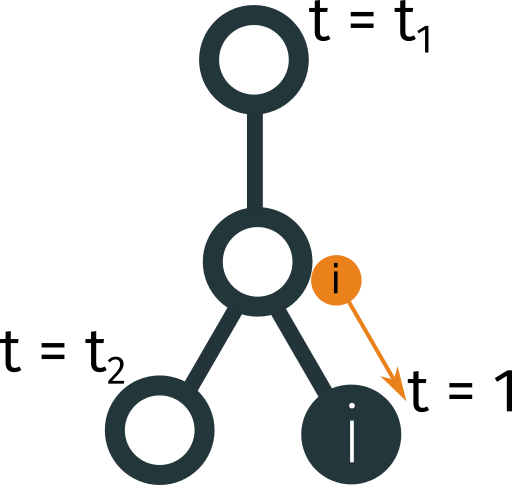
\includegraphics[width=0.18\textwidth]{img/ddt-5}
  %\end{center}

  %\pause

  %If $a(1) = \infty$, each particle is guaranteed to diverge before $t = 1$.

%\end{frame}

%\begin{frame}{Generalizations}
  %\begin{center}
    %\includegraphics<1>[width=0.8\textwidth]{img/tree-graph-0}
    %\includegraphics<2>[width=0.8\textwidth]{img/tree-graph-1}
    %\includegraphics<3>[width=0.8\textwidth]{img/tree-graph-2}
    %\includegraphics<4>[width=0.8\textwidth]{img/tree-graph-3}
    %\includegraphics<5>[width=0.8\textwidth]{img/tree-graph-4}
    %\includegraphics<6>[width=0.8\textwidth]{img/tree-graph-5}
    %\includegraphics<7>[width=0.8\textwidth]{img/tree-graph-6}
    %\includegraphics<8>[width=0.8\textwidth]{img/tree-graph-7}
  %\end{center}
%\end{frame}

%\begin{frame}{Tree likelihood models}
  %Now, given a sample from a tree prior (assume a
  %cladogram with ordering and times),
  %we need to generate a dataset.

  %\begin{center}
    %\includegraphics<1>[width=\textwidth]{img/tree-data-0}
    %\includegraphics<2>[width=\textwidth]{img/tree-data-1}
  %\end{center}

%\end{frame}

%\begin{frame}{Latent tree parameters}
  %For every internal node in the tree $n$
  %we associate a latent parameter $\theta_n$
  %which is in the same space as the data.

  %\begin{center}
    %\includegraphics<2->[width=0.35\textwidth]{img/tree-4-parameters}
  %\end{center}

  %\pause

  %We then define:
  %\begin{itemize}
    %\item<3-> A prior distribution $P_0(\theta)$
    %\item<4-> A transition kernel $T(\theta' | \theta)$
  %\end{itemize}

%\end{frame}

%\begin{frame}{Example likelihood models}
  %The most common likelihood model is \alert{Brownian motion},
  %also called Gaussian diffusion, which is
  %\begin{align}
    %P_0(\theta) &= \mathcal{N}(0, \sigma_0^2I) \\
    %T(\theta' | \theta) &= \mathcal{N}(\theta, \sigma^2(t - t')),
  %\end{align}
  %where $t$ and $t'$ are the times associated with nodes
  %$\theta$ and $\theta'$ and $\sigma_0^2$ and $\sigma^2$ are hyperparameters.

  %\pause

  %Other options are:
  %\begin{itemize}
    %\item Multinomial-Dirichlet diffusion: useful for
      %categorical data
    %\item Multinomial diffusion: useful for
      %counts (such as bag-of-words)
  %\end{itemize}
%\end{frame}

%\begin{frame}{Sampling latent variables}
  %We are interested in sampling $P(T, \theta | X)$.
  %\begin{itemize}
    %\item Define tree proposal
      %$q_\mathcal{T}(T' | T)$
    %\item Define parameter proposal $q_\Theta(\theta' | T', \theta)$.
  %\end{itemize}

  %\uncover<2->{\textbf{Tree proposal:} \alert{subtree-prune and regraft} (SPR) move}

  %\begin{center}
    %\includegraphics<2>[width=\textwidth]{img/spr-1}
    %\includegraphics<3>[width=\textwidth]{img/spr-2}
    %\includegraphics<4->[width=\textwidth]{img/spr-3}
  %\end{center}

  %\uncover<5->{\textbf{Parameter proposal:} Gibbs sampling or marginalization}

%\end{frame}

%\section{Adding interaction}

%\begin{frame}{Why interaction?}
  %Recall the motivating example for Bayesian hierarchical clustering.
  %\begin{center}
  %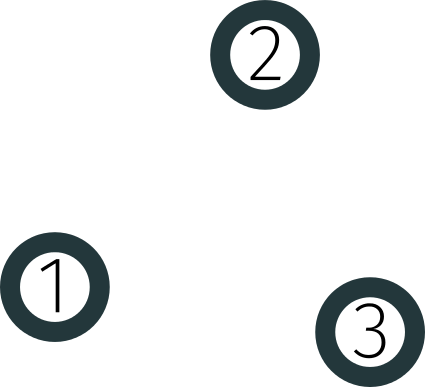
\includegraphics[width=0.3\textwidth]{img/3-cluster}\hfill
  %\includegraphics[width=0.45\textwidth]{img/3-cluster-line}
  %\end{center}
  %Could a user provide feedback and help decide which hierarchy
  %makes the most sense?
  %\begin{itemize}
    %\item Interactive Bayesian Hierarchical Clustering - Vikram and Dasgupta (2016) \cite{Vikram2016}
  %\end{itemize}
%\end{frame}

%\begin{frame}{Interactive hierarchical clustering}
  %\begin{center}
    %\includegraphics<1>[width=\textwidth]{img/interaction-0}
    %\includegraphics<2>[width=\textwidth]{img/interaction-1}
    %\includegraphics<3>[width=\textwidth]{img/interaction-2}
    %\includegraphics<4>[width=\textwidth]{img/interaction-3}
  %\end{center}
%\end{frame}

%\begin{frame}{Subtree queries}
  %Two main ideas:
  %\pause
  %\metroset{block=fill}
  %\begin{block}{Enforcing constraints}
    %To enforce constraints, we use
    %a modified SPR move that avoids
    %regraft branches that violate constraints.
  %\end{block}
  %\pause
  %\metroset{block=fill}
  %\begin{block}{Intelligent subset queries}
    %We pick subsets of data that have high variance,
    %which we can measure using samples.
  %\end{block}
%\end{frame}

%\begin{frame}{Results}
  %\begin{figure}
    %\centering
    %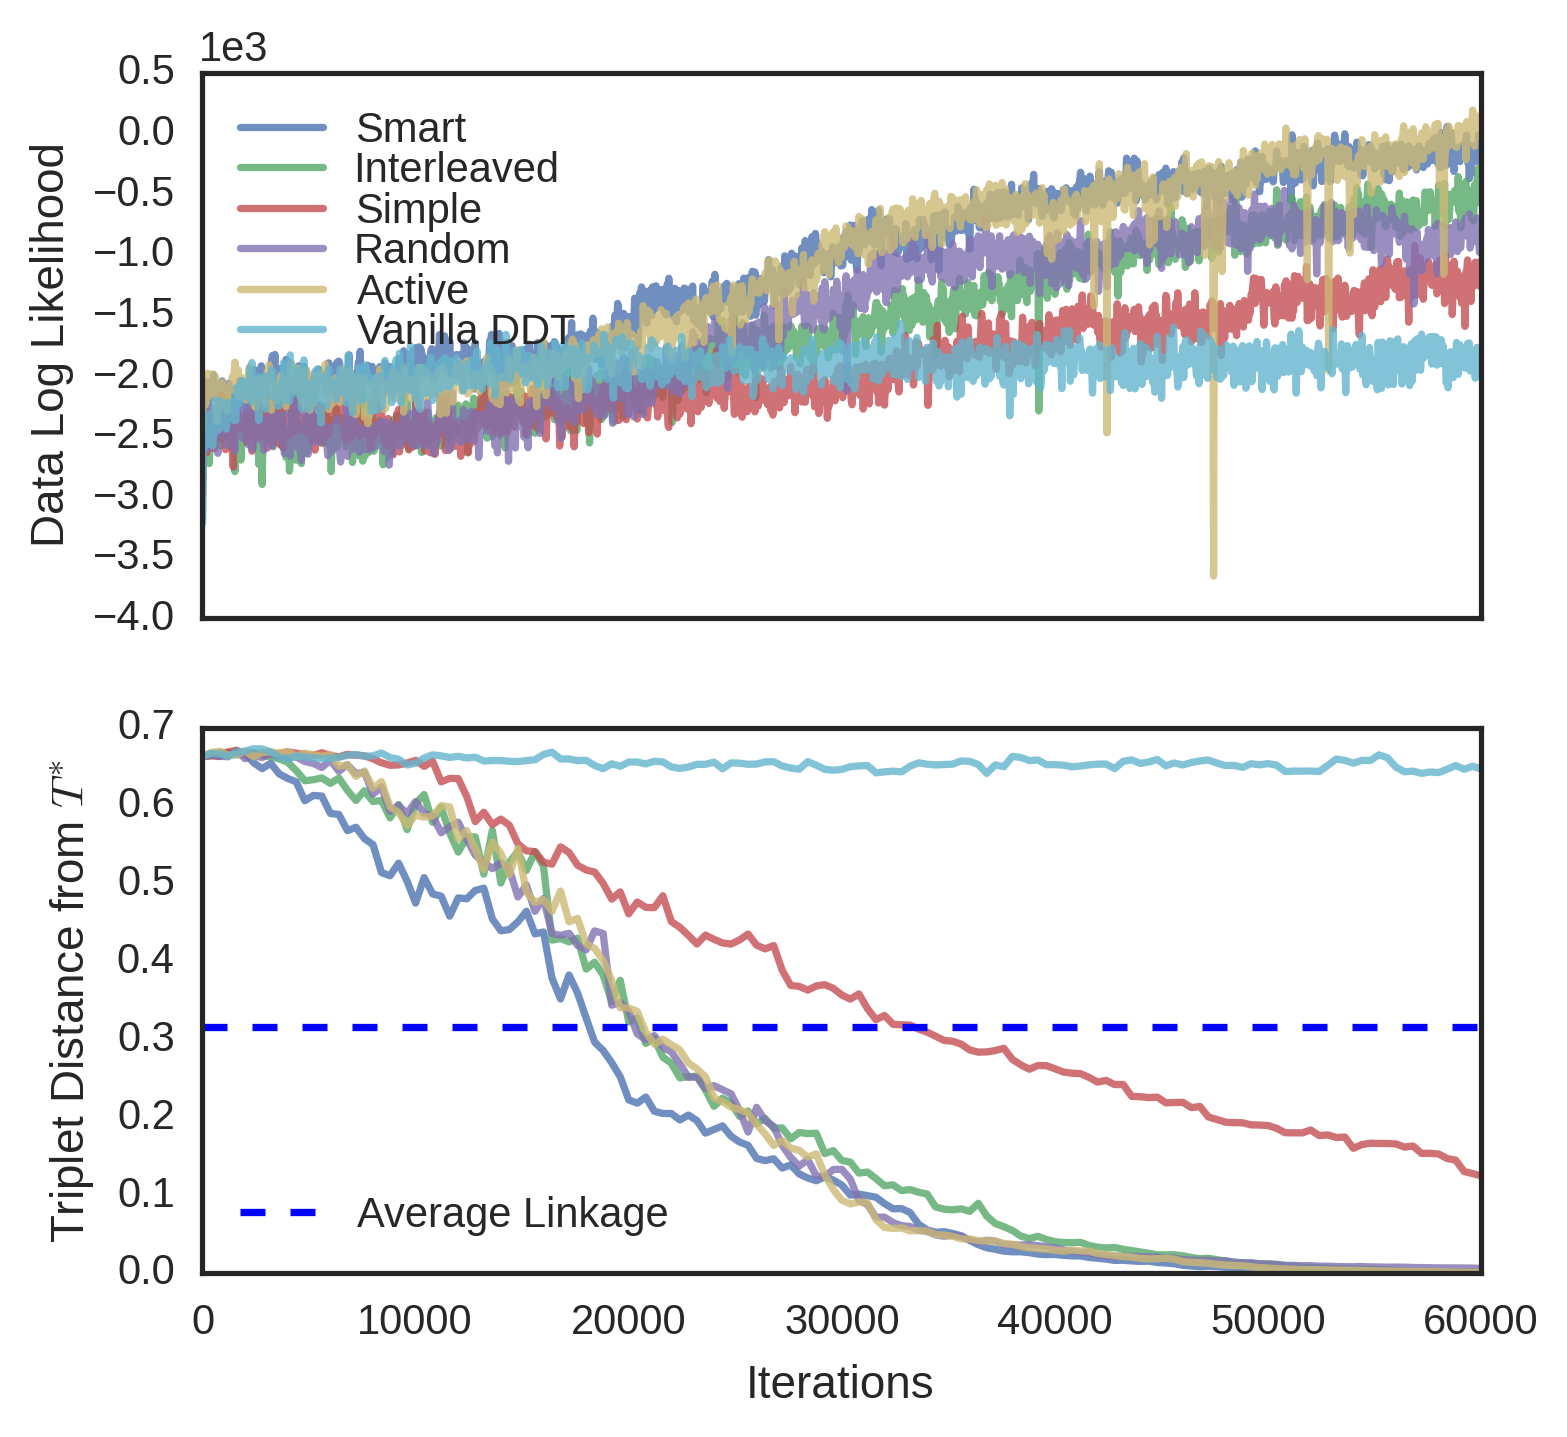
\includegraphics[frame, width=0.6\textwidth]{img/interactive}
    %\caption{The results of interactive Bayesian hierarchical clustering
    %on a dataset of zoo animals. Pictured are the
    %data log likelihood and percentage of triplets
    %satisfied for several subset querying methods. Source: \cite{Vikram2016}}
    %\label{fig:ibhc}
  %\end{figure}
%\end{frame}
%\section{Conclusion}

%\begin{frame}{Summary}
  %\begin{itemize}
    %\item<1-> Bayesian hierarchical clustering (BHC) is a general framework
      %in unsupervised learning that naturally handles
      %ambiguity and uncertainty in data.
    %\item<2-> BHC models can be decomposed into prior distributions
      %on trees, and likelihood models. Tree priors
      %can further be decomposed into
      %coalescent and diffusion models.
    %\item<3-> Inference in BHC can be performed
      %with MCMC methods like Metropolis-Hastings
      %using the subtree-prune and regraft move.
    %\item<4-> BHC enables
      %incorporating user interaction
      %into hierarchical clustering.
  %\end{itemize}
%\end{frame}

%\begin{frame}{Future work}
  %\begin{itemize}
    %\item<1-> \textbf{How can we improve on interactive Bayesian hierarchical clustering?}
      %Robust constraints, more tree priors, other measures of variance
    %\item<2-> \textbf{What is the effect of interaction in Bayesian problems?}
      %constrained posterior distributions, complexity of inference
    %\item<3-> \textbf{How can we extend interactive methods
      %to other domains?} metric learning, deep learning,
      %embeddings
  %\end{itemize}
%\end{frame}

%\begin{frame}[standout]
%Questions?
%\end{frame}

%\begin{frame}[allowframebreaks]{References}
  %\bibliography{main}
  %\bibliographystyle{unsrt}
%\end{frame}
\end{document}
